Given the restricted application domain of PaaS-hosted web APIs, we believe
that it is possible to design a system that predicts response time SLAs for
them using only static information from the web API code itself.  To enable
this, we design Cerebro with three primary components:
\begin{itemize}
\item A static analysis tool that extracts sequences of cloud SDK operations for 
each path through a method (web API operation),
\item A monitoring agent that runs in the target PaaS, and efficiently monitors 
the performance of the underlying cloud SDK operations, and
\item A prediction mechanism that uses the outputs of these two components to accurately predict an upper bound on the execution time of the web API.
\end{itemize}
We overview each of these components in the subsections that follow and then 
present the Cerebro workflow with an example.

\subsection{Static Analysis}
 This component analyzes the source code of the web API
(or some intermediate representation of it) and extracts a sequence of cloud API operations.
We implement our analysis for Java bytecode programs
using the Soot framework~\cite{Vallee-Rai:2010:SJB:1925805.1925818}.
Currently, our prototype analyzer considers the 
following Java codes as exposed web APIs.
\begin{itemize}
\item classes that extend the \textit{javax.servlet.HttpServlet} class (i.e. Java servlet implementations)
\item classes that contain JAXRS \textit{@Path} annotations, and
\item any other classes explicitly specified by the developer in a special configuration file.
\end{itemize}

Cerebro performs a simple construction and inter-procedural static analysis 
of control flow graph 
(CFG)~\cite{Allen:1970:CFA:800028.808479,Aho:1986:CPT:6448,Morgan:1998:BOC:288765,Muchnick:1998:ACD:286076} for each web API operation.
The algorithm extracts all cloud SDK operations along
each path through the methods. Cerebro analyzes calls to other functions
that the method calls, recursively.  Cerebro caches cloud SDK details for each function 
once analyzed so that it can be reused efficiently for other call sites to the same
function. Cerebro does not analyze third-party library calls, if any 
(which in our experience typically do not contain cloud SDK calls). Cerebro encodes
each cloud SDK call sequence for each path in a lookup table. We identify
cloud SDK calls by their Java package name (e.g. \texttt{com.google.appengine.apis}).

To handle loops, we first extract them from the CFG and 
annotate all cloud SDK invocations that occur within them.
We annotate each such SDK invocation with an estimate on the number of times
the loop is likely to execute in the worst case. 
We estimate loop bounds using a loop bound prediction algorithm 
based on abstract interpretation~\cite{bygde2010static}. 

As shown in the previous section, loops in these programs 
are rare and, when they do occur, they are
used to iterate over a data set returned from a database.
For such data dependent loops, we estimate the bounds if specified 
in the cloud SDK call (e.g. the maximum number of 
entities to return~\cite{gae-fetch-options}).
If our analysis is unable to estimate the bounds for these loops, Cerebro prompts
the developer for an estimate of the likely data set size and/or loop bounds.

\subsection{PaaS Monitoring Agent}
Cerebro monitors and records the response time of individual
cloud SDK operations within a running PaaS system.  Such support can be 
implemented as a PaaS-native feature or as
a PaaS application (web API); we use the latter in our prototype.
The monitoring agent runs in the background with, but separate from, 
other PaaS-hosted web APIs.
The agent invokes cloud SDK operations periodically on synthetic data sets and 
records timestamped response times in the PaaS datastore for each cloud SDK
operation.
Finally, the agent periodically reclaims old measurement data
to eliminate unnecessary storage. The Cerebro monitoring and reclamation 
rates are configurable and monitoring benchmarks can be added and customized
easily to capture common PaaS-hosted web API coding patterns.

In our prototype, the agent monitors the datastore and memcache services
every 60 seconds. In addition, it 
benchmarks loop iteration over datastore entities to capture
the performance of iterative datastore reads for datastore result set sizes 
of 10, 100, and 1000. We limit ourselves to these values because the PaaS requires
that all operations complete (respond) within 60 seconds -- so the data
sizes returned are typically small.

\subsection{Making SLA Predictions}
\label{sec:qbets}
To make SLA predictions, Cerebro uses 
Queue Bounds Estimation from Time Series (QBETS)~\cite{Nurmi:2007:QQB:1791551.1791556},
a non-parametric time series analysis method that we developed in prior work.
We originally designed QBETS for
predicting the scheduling delays for the batch queue systems 
used in high performance computing environments. 
We adapt it herein for use ``as-a-service'' in PaaS systems 
to predict the execution time of web APIs.

A QBETS analysis requires three inputs:
\begin{enumerate}
\item A time series of data generated by a continuous experiment.
\item The percentile for which an upper bound should be predicted ($p \in [1..99]$).
\item The upper confidence level of the prediction ($c \in (0,1)$).
\end{enumerate}

QBETS uses this information to predict an upper bound for 
the $p^{th}$ percentile of the time series.  It does so by treating each
observation as a Bernoulli trial with probability $0.01p$ of succeess.  Let $q
= 0.01p$.  Then if there are $n$ observations, the probability of there being
exactly $k$ successes is described by a Binomial distribution (assuming
independence of the observations)
having parameters $n$ and $q$.  If $Q$ is the $p^{th}$ percentile of the
distribution from which the observations have been drawn, the equation 
\vspace{-0.1in}
\begin{equation}\label{sumformula}
1 - \sum_{j=0}^k { n \choose j } \cdot (1-q)^{j} \cdot q^{n-j}
\end{equation}
gives the probability that more that $k$ obervations are greater than $Q$.
As a result, the $k^{th}$ largest value in a sorted list of $n$ observations
gives an upper $c$ confidence bound on $Q$ when $k$ is the smallest integer
value for which Equation~\ref{sumformula} is larger than $c$.

More succinctly, QBETS sorts the observations in a history of observations,
and computes the value of $k$ that constitutes an index into 
this sorted list of the observation that is the upper $c$ confidence bound on
the $p^{th}$ percentile. The methodology assumes that the time series of 
observations is 
ergodic so that, in the long run, the confidence bounds are accurate.  

QBETS also attempts to detect change points in the time series of observations 
so that it can apply this inference technique to only the most recent 
segment of the series that appears to be stationary.  
To do so, it compares
percentile bounds predictions with observations throughout the series and
determines where thes series is likely to have undergone a change.  It then
discards observations from the series prior to this change point and
continues.  As a result, when QBETS starts, it must ``learn'' the series by
scanning it in time series order to determine the change points.  We discuss
the learning time for the data we have gathered in this study in
Subsection~\ref{sec:learning}.

%The predicted value has a probability of $0.01p$ of 
%being greater than or equal to the next data point that
%will be added to the time series by the continuous experiment. 
%The upper confidence level $c$ serves as a conservative
%bound on the predictions. That is, predictions made with an upper confidence 
%level of $c$ will overestimate
%the true percentile with a probability of $1-c$. This confidence guarantee 
%is necessary because QBETS does not determine the 
%percentiles of the time series precisely, but only estimates them. 
%If not provided as part of Cerebro invocation, our prototype 

Note that $c$ is an upper confidence level on $p^{th}$ percentile
which makes the QBETS
bound estimates conservative.  That is, the value returned by QBETS as a bound
prediction is larger than the true $p^{th}$ percentile with probability $1-c$
under the assumptions of the QBETS model. 
In this study, we use the $95^{th}$ percentile and $c = 0.01$ unless
otherwise stated. 

Note that the algorithm itself can be implemented efficiently so that it is
suitable for on-line use.  Details of this implementation as well as a fuller
accounting of the statistical properties and assumptions are available
in~\cite{Nurmi:2007:QQB:1791551.1791556,uptime-bootstrap,quant-est,ckpt-sched}.

%defaults to $p=95$ and $c=0.05$. 

%For example, assume a continuous experiment 
%in which we periodically measure the
%response time of a web API. Doing so results in a time series of 
%response time data. Suppose at time $t$,
%we run QBETS on the time series data collected so far 
%with $p=95$ and $c=0.01$. The prediction returned
%by QBETS has a 95\% chance of being greater than or equal 
%to the next response time value measured
%by our experiment after time $t$. Since $c=0.01$, the predicted value has a 99\% chance of
%overestimating the true 95th percentile of the time series.

QBETS requires a sufficiently large number of data points
in the input time series before it can make an accurate prediction. 
Specifically, the largest value in a sorted list of $n$ observations is
greater than the $p^{th}$ percentile with confidence $c$ when $n >=
log(c)/log(0.01p)$.

For example, predicting the $95^{th}$ percentile
of the API execution time, with an upper confidence of $0.01$ requires at
least $90$ observations.
We use this information to control 
reclamation of monitoring data in the cloud SDK monitoring agent.

\subsection{Example Cerebro Workflow}

\begin{figure}
\centering
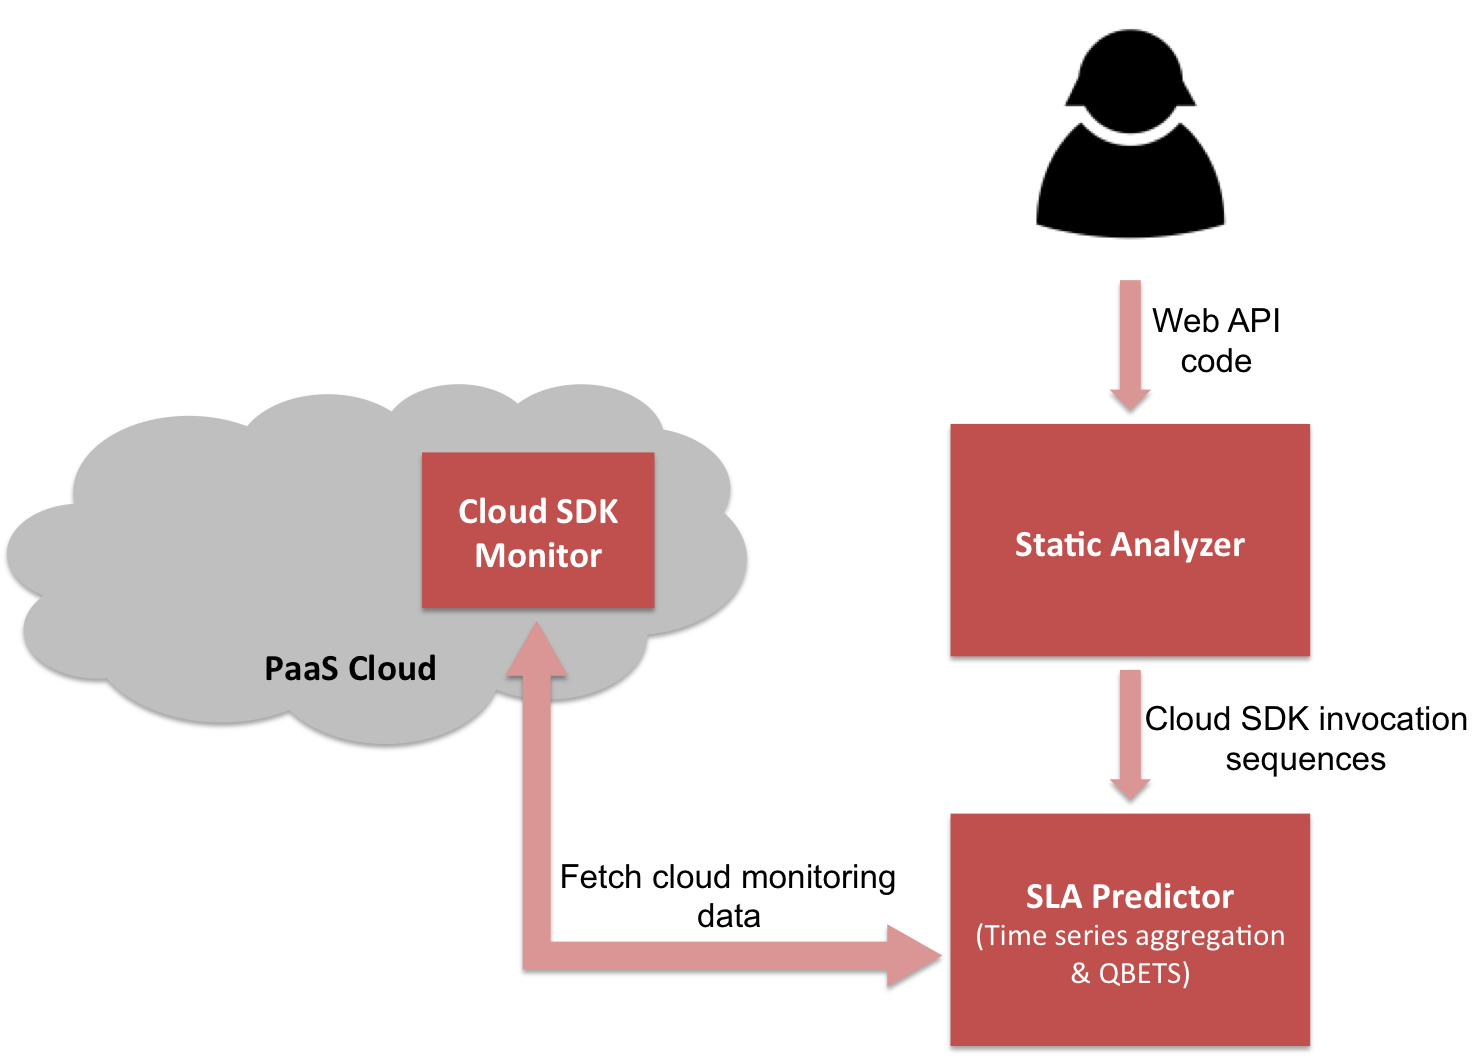
\includegraphics[scale=0.35]{cerebro_arch}
\caption{Cerebro architecture and component interactions.}
\label{fig:cerebro_arch}
\end{figure}

Figure~\ref{fig:cerebro_arch} illustrates how the Cerebro components interact with
each other during the prediction making process.  Cerebro can be
invoked when a web API is deployed to a PaaS cloud or at any time during the development
process to give developers insight into the worst case response time of their
applications.

Upon invoking Cerebro with a web API code, Cerebro
performs its static analysis on all operations in the API. For each
analyzed operation it produces a list of annotated cloud SDK invocation sequences --
one sequence per program path. Cerebro then prunes this list to eliminate duplicates.
Duplicates occur when a web API operation has
multiple program paths with the same sequence of cloud SDK invocations.
Next, for each pruned list Cerebro performs the following operations:
\begin{enumerate}
\item Retrieve (possibly compressed) benchmarking data from the monitoring agent 
for all SDK operations in each sequence. The agent returns
ordered time series data (one time series per cloud SDK operation).
\item Align retrieved time series across operations in time, and sum the aligned
values
to form a single \textit{joint} time series of the summed values for the 
sequence of cloud SDK operations.
\item Run QBETS on the aggregate time series with the 
desired $p$ and $c$ values to predict an upper bound. 
\end{enumerate}
Cerebro uses largest predicted value (across path sequences and operations) 
as its SLA prediction for the web API.
This process (SLA prediction) can be implemented
as a co-located service in the PaaS cloud or as a standalone utility.  We do 
the latter in our prototype.

As an example, suppose that the static analysis results in the
cloud SDK invocation sequence $<op_{1},op_{2},op_{3}>$ for
some operation in a web API. 
Assume that the monitoring agent has collected the following
time series for the three SDK operations:
\begin{itemize}
\item $op_{1}$: $[t_{0}: 5, t_{1}: 4, t_{2}: 6, ...., t_{n}: 5]$
\item $op_{2}$: $[t_{0}: 22, t_{1}: 20, t_{2}: 21, ...., t_{n}: 21]$
\item $op_{3}$: $[t_{0}: 7, t_{1}: 7, t_{2}: 8, ...., t_{n}: 7]$
\end{itemize}

Here $t_{m}$ is the time at which the $m^{th}$ measurement is taken.
Cerebro aligns the three time series according to timestamps, 
and sums the results
to obtain the following joint time series:
$[t_{0}: 34, t_{1}: 31, t_{2}: 35, ...., t_{n}: 33]$

If any operation is tagged as being inside a loop, where the loop
bounds have been estimated, Cerebro multiplies
the time series data corresponding to that 
operation by the loop bound estimate before aggregating. In cases where the operation 
is inside a data dependent loop, we request the time series data from 
the monitoring agent for its iterative datastore read benchmark 
for a number of entities that is equal to or larger than the annotation
and include it in the joint time series.

Cerebro passes the final joint
time series for each sequence of operations to QBETS, 
which returns the worst-case upper bound response time it predicts.
If the QBETS predicted value is $Q$ milliseconds, 
Cerebro forms the SLA as ``the web API will respond  in
under $Q$ milliseconds, $p$\% of the time''. 
When the web API has multiple operations, Cerebro estimates multiple 
SLAs for the API. 
If a single value is needed for the entire API regardless of operation,
Cerebro returns the largest 
predicted value as the final SLA (i.e. the worst case SLA for the API).

%Cerebro allows PaaS administrators to define API governance policies that 
%allow an application to be deployed only when its web APIs will meet a 
%pre-determined (or pre-negotiated) SLA target and to be notified 
%by the platform when such SLAs require renegotiation.


%this should go in the evaluation (where we discuss correctness), not here
%The QBETS implementation we use does not just generate one prediction when executed on
%some input time series. Rather, it generates a sequence of predictions -- one prediction per data point in the input
%time series. That is, it provides a trace of how the predictions change with each observed data point.
%When run on time series data gathered by our cloud SDK monitor,
%this would result in a prediction sequence with one entry per minute.
%We return the entire sequence of predictions generated by QBETS
%as the output. In situations where we just need a single prediction value, we pick the last prediction of the output
%sequence, and discard the rest.
